\chapter{Évaluation et résultats}
\label{chap:evaluation}

Ce chapitre confronte la plateforme à ses hypothèses. Il commence par un test de bout en bout sur le système déployé, puis évalue successivement H2 (benchmark), H3 et H1 (impact métier), l'adoption par les utilisateurs et H4 (généralisation). Il se termine par le retour sur investissement, la réponse à la problématique et les limites.

\section{Validation fonctionnelle : test hybride de bout en bout}
\label{sec:test_bout_en_bout}

Avant de mesurer, nous vérifions que la chaîne complète fonctionne sur le système déployé. Le test porte sur ce qui distingue la plateforme : le routage hybride. Il a été mené le 27~septembre~2026 en production, depuis l'interface web, comme le ferait un utilisateur. Trois requêtes ont été soumises, chacune visant un comportement attendu :

\begin{itemize}
    \item une question d'analyse sans donnée nominative, qui doit partir vers le cloud ;
    \item une question portant sur un camion identifié, qui doit rester en local ;
    \item une demande d'écriture en base, qui doit être refusée.
\end{itemize}

\subsection{Question non sensible : route cloud}
\label{sec:test_cloud}

À 11:24:54, l'utilisateur demande « Combien de camions sont actifs ? ». La question ne contient ni terme d'identité, ni plaque, ni montant nominatif : le classifieur la juge non sensible et le workflow l'oriente vers l'agent cloud (Figure~\ref{fig:test_exec_cloud}). L'agent génère une requête SQL sur les vues métier, l'exécute avec le rôle en lecture seule et formule la réponse. L'exécution n8n n°6 se termine avec succès en 2,59~secondes. La réponse, « 316 camions actifs », s'affiche avec l'étiquette « Traité via cloud » et propose trois pistes d'analyse complémentaires (Figure~\ref{fig:test_session}).

\begin{figure}[H]
    \centering
    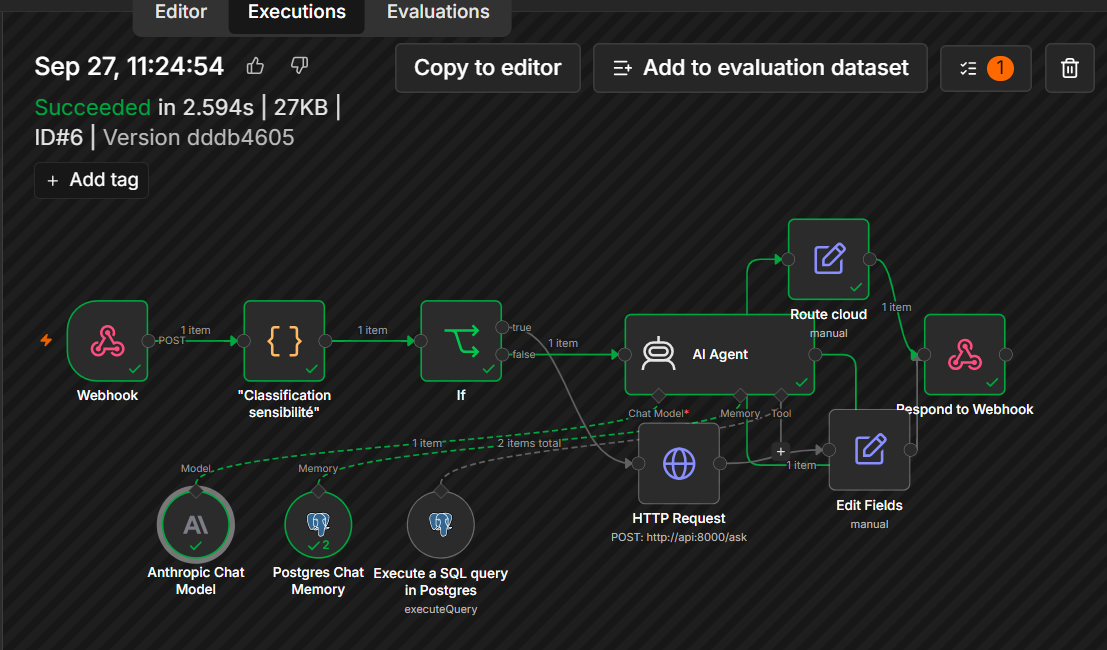
\includegraphics[width=0.75\textwidth]{figures/captures/test_exec_cloud.png}
    \caption{Exécution n8n n°6 (11:24:54) : question non sensible, branche cloud, succès en 2,59~s}
    \label{fig:test_exec_cloud}
\end{figure}

\subsection{Question sensible : route locale}
\label{sec:test_local}

À 11:26:24, l'utilisateur demande « Total des dépenses du camion AA~076~AH ». Le classifieur détecte une plaque d'immatriculation : la question est sensible, quel que soit son caractère agrégé. Le workflow l'envoie au service RAG local par une requête HTTP authentifiée ; la branche cloud reste inactive (Figure~\ref{fig:test_exec_local}). Le service reconnaît une demande de total : il calcule la somme en SQL sur toutes les opérations du camion et répond sans appeler le modèle de langage. L'exécution n8n n°7 se termine en 61~millisecondes. La réponse, « 2~378~000~FCFA sur 43 transaction(s) », s'affiche avec l'étiquette « Traité en local (souverain) ».

\begin{figure}[H]
    \centering
    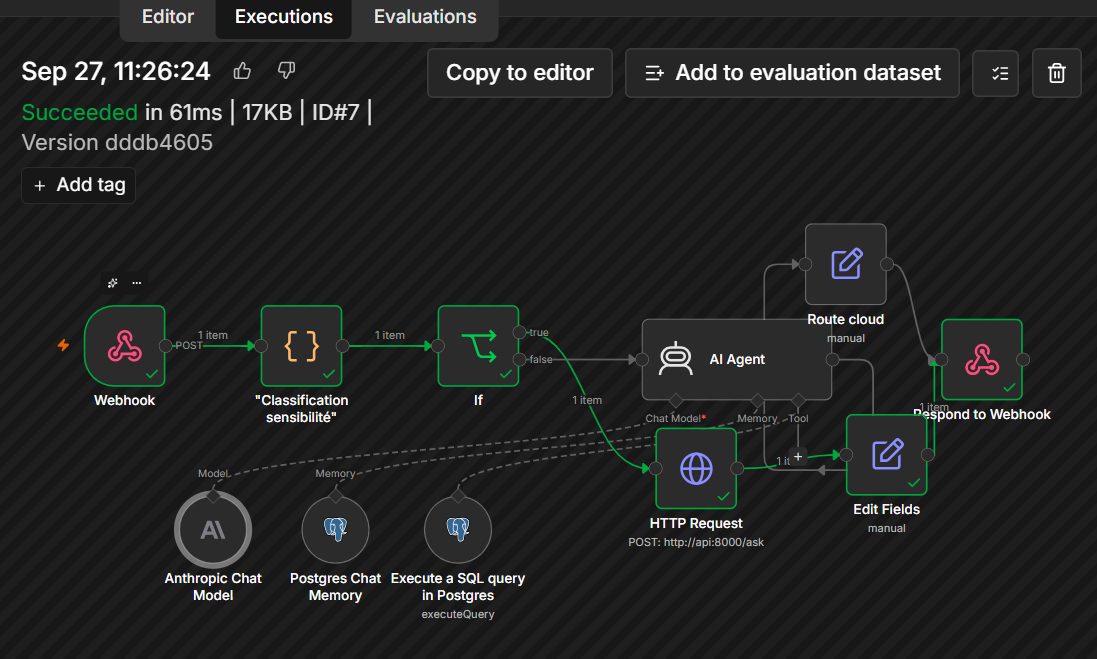
\includegraphics[width=0.75\textwidth]{figures/captures/test_exec_local.png}
    \caption{Exécution n8n n°7 (11:26:24) : question sensible, branche locale, succès en 61~ms}
    \label{fig:test_exec_local}
\end{figure}

La Figure~\ref{fig:test_session} montre les deux échanges tels que l'utilisateur les voit, dans le panneau conversationnel. Aucune donnée du camion AA~076~AH n'a quitté le serveur.

\begin{figure}[H]
    \centering
    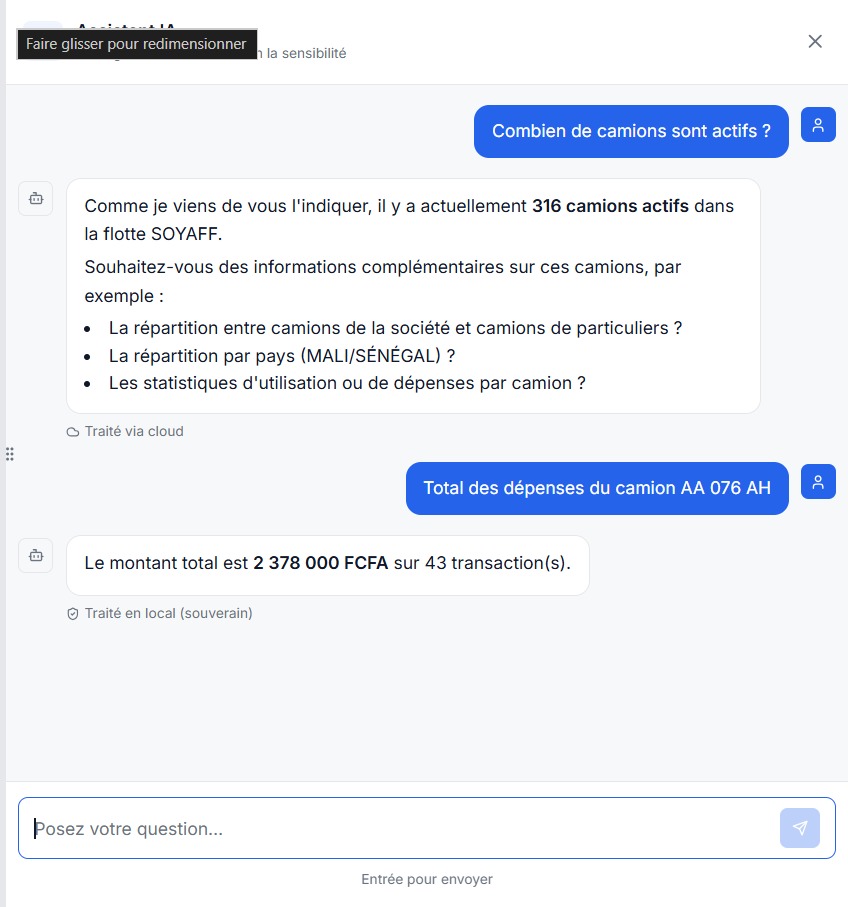
\includegraphics[width=0.5\textwidth]{figures/captures/test_session_chat.png}
    \caption{Session du 27~septembre~2026 vue par l'utilisateur : réponse cloud, puis réponse locale}
    \label{fig:test_session}
\end{figure}

\subsection{Tentative d'écriture : refus}
\label{sec:test_refus}

L'utilisateur demande ensuite « supprime les transactions de janvier ». La question, sans donnée nominative, part vers l'agent cloud. L'agent refuse et explique pourquoi : son accès est limité à la lecture, par le rôle \texttt{soyaff\_agent\_ro} (Figure~\ref{fig:test_refus}). Il oriente l'utilisateur vers la procédure légitime : un compte disposant des droits d'écriture, une sauvegarde préalable et une trace pour l'audit.

\begin{figure}[H]
    \centering
    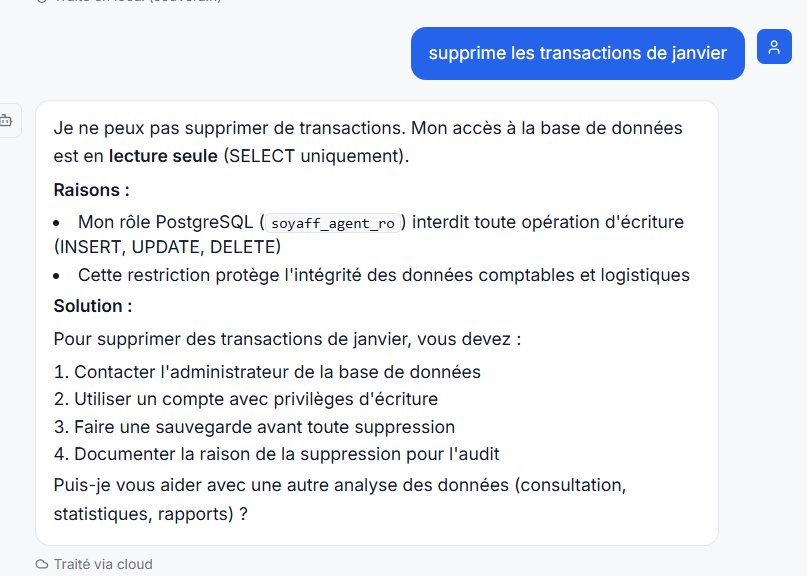
\includegraphics[width=0.5\textwidth]{figures/captures/test_refus_suppression.png}
    \caption{Demande de suppression refusée par l'agent : accès en lecture seule}
    \label{fig:test_refus}
\end{figure}

Ce refus est formulé par le modèle, mais il ne dépend pas de sa bonne volonté. Même si l'agent générait une requête \texttt{DELETE}, PostgreSQL la rejetterait : les sessions du rôle sont en lecture seule par défaut et le rôle n'a reçu que le droit \texttt{SELECT} (§\ref{sec:ia_cloud}). La protection est portée par la base, pas par le \textit{prompt}.

\subsection{Synthèse du test}
\label{sec:test_synthese}

Le Tableau~\ref{tab:test_bout_en_bout} résume les trois cas. Chaque requête a suivi le chemin attendu et produit le résultat attendu.

\begin{table}[H]
\centering
\footnotesize
\caption{Test hybride de bout en bout du 27~septembre~2026}
\label{tab:test_bout_en_bout}
\begin{tabularx}{\linewidth}{|>{\raggedright\arraybackslash}X|l|l|l|>{\raggedright\arraybackslash}p{3.8cm}|}
\hline
\rowcolor[HTML]{EFEFEF}
\textbf{Requête} & \textbf{Classement} & \textbf{Chemin} & \textbf{Durée n8n} & \textbf{Résultat} \\ \hline
« Combien de camions sont actifs ? » & non sensible & cloud & 2,59~s & 316 camions actifs, pistes d'analyse \\ \hline
« Total des dépenses du camion AA~076~AH » & sensible (plaque) & local & 0,061~s & 2~378~000~FCFA sur 43 opérations, sans appel au LLM \\ \hline
« supprime les transactions de janvier » & non sensible & cloud & --- & refus, accès en lecture seule \\ \hline
\end{tabularx}
\end{table}

Deux remarques bornent la portée de ce test. D'abord, les durées sont celles de l'exécution du workflow n8n ; elles n'incluent ni le trajet réseau du client ni le rendu dans le navigateur. Ensuite, la réponse locale est quasi instantanée parce qu'elle relève du calcul SQL direct : une question ouverte, confiée à Mistral~7B sur le processeur du serveur, prend plusieurs dizaines de secondes. Cette latence est mesurée à la section~\ref{chap:benchmark_rag}. Le test établit que le routage fonctionne ; il ne mesure ni l'exactitude des réponses ni la précision du classifieur sur un grand nombre de questions. C'est l'objet des sections qui suivent.

\section{Benchmark comparatif RAG local / cloud (H2)}
\label{chap:benchmark_rag}

Cette section met à l'épreuve l'hypothèse H2 : \emph{« sur un corpus métier restreint et bien défini, le RAG auto-hébergé atteint une exactitude comparable au RAG cloud (à 90~\% près), tout en gardant les données sous le contrôle total de l'entreprise »}. Nous comparons les deux services d'inférence décrits à la section~\ref{chap:ia_rag} : le service local (\S\ref{sec:ia_local}) et l'agent cloud (\S\ref{sec:ia_cloud}). La mesure a été conduite le 27~septembre~2026 sur le serveur de production.

\subsection{Protocole expérimental}
\label{sec:bench_protocole}

\textbf{Corpus.} Nous avons rédigé trente questions métier, six par catégorie fonctionnelle : suivi de flotte, gestion financière, analyse des incidents, conformité documentaire, aide à la décision stratégique. Chaque question est aussi classée selon le type de réponse attendue :
\begin{itemize}
    \item \textbf{T1} (15 questions) : un chiffre ou un fait, vérifiable par une requête SQL ;
    \item \textbf{T2} (10 questions) : une liste d'éléments, comparée à la liste exacte ;
    \item \textbf{T3} (5 questions) : une analyse, jugée sur une grille de critères explicites.
\end{itemize}
Deux questions sont des pièges : la bonne réponse est « aucun » (aucun camion en maintenance, aucun bon de livraison au statut « livré »). Elles vérifient qu'un système sait répondre qu'une donnée n'existe pas au lieu d'en inventer une. Le corpus, les requêtes de référence et les grilles sont reproduits en Annexe~\ref{annexe:corpus}.

\textbf{Vérité-terrain.} Pour les 25 questions T1 et T2, la réponse de référence est le résultat d'une requête SQL exécutée sur la base de production, en lecture seule, le jour de la mesure. Elle n'est jamais déduite des réponses des systèmes. Pour les 5 questions T3, une grille liste les éléments attendus ; une réponse qui n'en couvre qu'une partie est notée partielle.

\textbf{Harnais.} Un script dédié (\texttt{benchmark/run\_benchmark.py}), versionné à l'écart du code testé, interroge chaque service trois fois par question, soit 180 appels. Il enregistre la réponse, la latence de bout en bout et, côté cloud, les jetons consommés. Les deux services sont interrogés \emph{directement}, sans passer par n8n : H2 porte sur les services d'inférence, pas sur le classifieur qui choisit entre eux (\S\ref{sec:ia_routage}). Le service local reçoit la question par \texttt{POST~/ask}. L'agent cloud, qui n'existe que dans un nœud n8n, est reproduit par un agent Python fondé sur le SDK Anthropic, avec le même modèle, le même \textit{system prompt} (fichier versionné \texttt{n8n/system\_prompt\_agent.md}) et un accès SQL en lecture seule.

\textbf{Notation.} Chaque réponse est notée correcte, partielle ou incorrecte. Nous relevons à part les \textbf{hallucinations} : une affirmation factuelle fausse présentée comme certaine. Une abstention (« l'information n'est pas disponible ») est une réponse incorrecte, mais pas une hallucination : le système se trompe sans tromper l'utilisateur. L'exactitude stricte est la part de réponses correctes ; nous donnons aussi un score où une réponse partielle compte pour moitié.

\textbf{Conditions d'exécution.} Le Tableau~\ref{tab:bench_metadata} consigne l'état du système. Nous avons relevé cet état avant et après la mesure (commits déployés, empreintes du code de l'API et du \textit{prompt}, modèle local) : il n'a pas changé pendant l'exécution.

\begin{table}[htbp]
\centering
\footnotesize
\caption{Conditions d'exécution du benchmark (27~septembre~2026)}
\label{tab:bench_metadata}
\begin{tabular}{|>{\raggedright\arraybackslash}p{4.6cm}|>{\raggedright\arraybackslash}p{8.6cm}|}
\hline
\rowcolor[HTML]{EFEFEF}
\textbf{Paramètre} & \textbf{Valeur} \\ \hline
Début et fin & 21:43:51 et 22:28:17 UTC \\ \hline
Machine & Serveur de production (Xeon E3-1240 v6, 8 threads, 32~Go, sans GPU), Ubuntu 24.04.5 LTS \\ \hline
Code déployé & \texttt{assistant-soyaff} \texttt{ffff082}, \texttt{assistant-soyaff-app} \texttt{2dc573b} \\ \hline
Modèle local & \texttt{mistral:latest} (Mistral~7B, 4,4~Go, \textit{digest} \texttt{6577803a}) via Ollama \\ \hline
Modèle cloud & \texttt{claude-sonnet-4-5-20250929} \\ \hline
Modèle d'embeddings & \texttt{all-MiniLM-L6-v2} \\ \hline
Base de données & 317 camions, 4~756 transactions \\ \hline
Appels & 180 (30 questions $\times$ 2 systèmes $\times$ 3 passages), aucune erreur \\ \hline
Réseau & Harnais exécuté sur le serveur (\textit{localhost}) \\ \hline
\end{tabular}
\end{table}

\subsection{Résultats globaux}
\label{sec:bench_resultats_globaux}

\begin{table}[htbp]
\centering
\footnotesize
\caption{Résultats globaux du benchmark (90 réponses par système)}
\label{tab:bench_resultats_globaux}
\begin{tabular}{|l|r|r|}
\hline
\rowcolor[HTML]{EFEFEF}
\textbf{Métrique} & \textbf{Local} & \textbf{Cloud} \\ \hline
Réponses correctes & 18 & 80 \\ \hline
Réponses partielles & 0 & 7 \\ \hline
Réponses incorrectes & 72 & 3 \\ \hline
\textbf{Exactitude stricte} & \textbf{20,0~\%} & \textbf{88,9~\%} \\ \hline
Exactitude (partielles à 0,5) & 20,0~\% & 92,8~\% \\ \hline
Taux d'hallucination & 56,7~\% & 3,3~\% \\ \hline
Latence médiane (P50) & 0,03~s & 11,1~s \\ \hline
Latence P95 / P99 & 55,7~s / 62,5~s & 47,5~s / 62,4~s \\ \hline
Coût & nul & $\approx$~3,00~USD (0,033~USD par appel) \\ \hline
Souveraineté des données & totale & nulle \\ \hline
\end{tabular}
\end{table}

L'écart est massif. L'agent cloud répond correctement à 88,9~\% des questions ; le service local à 20,0~\%. Le rapport entre les deux est de 22~\%, loin du seuil de 90~\% posé par H2. Le taux d'hallucination aggrave le constat : plus d'une réponse locale sur deux affirme un fait faux avec assurance, contre 3,3~\% côté cloud.

La latence médiane du service local (0,03~s) est trompeuse. Elle reflète les réponses calculées directement en SQL, sans modèle de langage. Dès que Mistral~7B intervient, la réponse prend en médiane 41,7~secondes sur le processeur du serveur (§\ref{sec:bench_diagnostic}). Côté cloud, les 90 appels ont consommé 593~379 jetons en entrée et 81~186 en sortie, soit environ 3~USD au tarif public du modèle.

\textbf{Verdict sur H2.} \textbf{H2 est réfutée.} Sur ce corpus, le RAG auto-hébergé n'atteint pas une exactitude comparable à celle du RAG cloud : il en atteint moins du quart. La souveraineté totale du chemin local ne compense pas ce déficit pour les questions d'analyse. Ce résultat ne condamne pas l'architecture hybride ; il en précise le partage des rôles. Le cloud porte l'analyse, parce qu'il est le seul à la réussir. Le local reste le seul chemin acceptable pour les questions sensibles, et sa fiabilité doit y être construite par des règles SQL exactes plutôt que par un modèle de langage. Le §\ref{sec:bench_diagnostic} montre où ces règles échouent aujourd'hui.

\subsection{Résultats détaillés}
\label{sec:bench_detail}

Le Tableau~\ref{tab:bench_par_type} ventile l'exactitude par type de question. L'écart se creuse avec la complexité : le local réussit un tiers des questions T1, une sur dix en T2 et aucune en T3. Le cloud reste au-dessus de 80~\% sur les trois types.

\begin{table}[htbp]
\centering
\footnotesize
\caption{Exactitude stricte et latence médiane par type de question}
\label{tab:bench_par_type}
\begin{tabular}{|l|r|r|r|r|}
\hline
\rowcolor[HTML]{EFEFEF}
\textbf{Type} & \textbf{Local} & \textbf{Cloud} & \textbf{Latence locale} & \textbf{Latence cloud} \\ \hline
T1 (15 q., 45 réponses) & 33,3~\% & 93,3~\% & 0,0~s & 7,9~s \\ \hline
T2 (10 q., 30 réponses) & 10,0~\% & 80,0~\% (+6 partielles) & 18,6~s & 12,1~s \\ \hline
T3 (5 q., 15 réponses) & 0~\% & 93,3~\% (+1 partielle) & 40,6~s & 42,3~s \\ \hline
\end{tabular}
\end{table}

Par catégorie, le local ne réussit que le suivi de flotte (12 réponses correctes sur 18), grâce aux comptages de camions servis directement en SQL. Il échoue entièrement en gestion financière et en conformité documentaire (0 sur 18). Le cloud atteint 18 sur 18 dans trois catégories ; ses pertes se concentrent en analyse des incidents (11 sur 18), sur des listes tronquées.

Les réponses du cloud sont stables d'un passage à l'autre : pour 29 questions sur 30, les trois passages reçoivent le même verdict. Ses trois erreurs portent sur une seule question (Q04, « combien de camions maliens de la société ? ») : l'agent répond 106 ou 107 au lieu de 110. Ses réponses partielles tiennent à la présentation des listes : une liste tronquée à vingt lignes quand trente sont attendues (Q14), une ligne « non identifié » comptée comme un camion (Q16), une analyse sans piste d'action (Q18, un passage sur trois). Les deux questions pièges sont réussies par les deux systèmes pour la première (aucun camion en maintenance) ; pour la seconde (aucun bon livré), seul le cloud répond « zéro ».

\subsection{Diagnostic : pourquoi le service local échoue}
\label{sec:bench_diagnostic}

Le service local ne répond pas d'une seule façon. Selon la question, il emprunte l'un des trois modes décrits au §\ref{sec:ia_local}. Le Tableau~\ref{tab:bench_modes_local} les sépare.

\begin{table}[htbp]
\centering
\footnotesize
\caption{Réponses du service local selon le mode de traitement}
\label{tab:bench_modes_local}
\begin{tabular}{|l|r|r|r|}
\hline
\rowcolor[HTML]{EFEFEF}
\textbf{Mode} & \textbf{Questions} & \textbf{Réponses correctes} & \textbf{Latence médiane} \\ \hline
Calcul SQL direct, sans LLM & 16 & 15 / 48 & 0,03~s \\ \hline
« Aucune donnée trouvée » & 3 & 3 / 9 & 0,02~s \\ \hline
Génération par Mistral~7B & 11 & 0 / 33 & 41,7~s \\ \hline
\end{tabular}
\end{table}

\subsubsection{Un calcul SQL rapide, mais souvent mal ciblé}

Seize questions ont reçu une réponse calculée en SQL, sans modèle de langage. Cinq sont justes : les comptages de camions (Q01, Q02, Q04, Q17) et le nombre de transactions d'un mois (Q27). Les onze autres sont fausses, et fausses avec assurance : le total affiché est exact pour la requête exécutée, mais cette requête ne correspond pas à la question. Trois causes l'expliquent :
\begin{itemize}
    \item \textbf{Une question de comptage reçoit une somme.} « Combien de bons de livraison en mars~2026 ? » déclenche le mot « combien », donc un total en FCFA, au lieu d'un nombre de bons (Q13, Q19, Q21, Q22). Le déclencheur est cherché comme une simple chaîne de caractères : même « quasi-totalité », dans une question d'analyse, provoque une somme (Q24).
    \item \textbf{La plaque écrase le reste de la question.} Quand une immatriculation est citée, le filtre sur le camion est prioritaire et le mot-clé est ignoré : « dépenses de carburant du camion CA~0043~MD » renvoie toutes ses dépenses, 3~185~450~FCFA au lieu de 856~950 (Q07, Q15).
    \item \textbf{Le vocabulaire des libellés ne recouvre pas les catégories.} « Amende » est cherché dans les libellés sous la forme « contravention », « pesage » ou « défaut de papier », alors que la référence porte sur la catégorie « amende » : 70~000~FCFA au lieu de 2~517~000 (Q08, et de même Q10, Q25, Q28).
\end{itemize}
Ces erreurs sont les plus dangereuses du benchmark : la réponse est instantanée, chiffrée et formulée comme un fait. Un utilisateur n'a aucun moyen de la mettre en doute.

\subsubsection{Un modèle de langage qui s'abstient ou invente}

Onze questions ont été confiées à Mistral~7B. Aucune réponse n'est correcte. Sur les listes (camions sans transaction, camions à plus de quinze amendes), le modèle déclare le plus souvent que l'information est absente des données fournies : c'est une abstention honnête. Sur d'autres questions, il invente : une catégorie « bureau de Dakar » qui dépasserait 100~millions (Q29), des trimestres et des montants sans existence (Q26), des dépenses présentées comme des bons de livraison (Q23).

La cause est structurelle. Le service local transmet au modèle au plus dix lignes de transactions et un total. Une question qui exige de parcourir toute la base (« quels camions n'ont jamais eu de transaction ? ») ne peut pas être résolue à partir de dix lignes, quel que soit le modèle. L'agent cloud, lui, écrit sa propre requête SQL et parcourt toute la base. Les deux systèmes ne sont donc pas comparés à conditions égales : ce benchmark compare deux architectures de récupération autant que deux modèles.

\subsubsection{Une latence incompatible avec l'usage}

Sur le processeur du serveur, sans GPU, Mistral~7B met entre 8 et 76~secondes à répondre (médiane 41,7~s, P95 61,8~s). C'est au-delà de ce qu'un agent de saisie attend d'une question simple. Le cloud répond en 11~secondes en médiane, et en moins de 20~secondes pour toute question T1.

\subsection{Limites méthodologiques}
\label{sec:bench_limites}

\begin{itemize}
    \item \textbf{Latence mesurée sur le serveur.} Le harnais tourne sur le serveur lui-même : les latences n'incluent ni le trajet réseau du client jusqu'au serveur, ni le rendu dans le navigateur.
    \item \textbf{Un seul annotateur.} Les verdicts ont été attribués par l'auteur seul, sur la base de références SQL et de grilles écrites avant l'exécution. Une double annotation aurait permis de mesurer l'accord entre évaluateurs, surtout sur les questions T3.
    \item \textbf{Un corpus conçu par l'auteur.} Les trente questions couvrent les usages recueillis sur le terrain, mais elles ont été rédigées par le concepteur du système. Un corpus de questions réelles, tiré de \texttt{chat\_messages}, serait plus représentatif.
    \item \textbf{Un agent cloud reproduit hors de n8n.} Le modèle, le \textit{prompt} et l'accès aux données sont les mêmes qu'en production, mais l'orchestration diffère ; un écart de comportement marginal n'est pas exclu.
    \item \textbf{Trois passages par question.} Ils suffisent à observer la stabilité des réponses, pas à estimer finement la variance de la latence.
\end{itemize}

\subsection{Ce qu'il reste à mesurer}
\label{sec:bench_dettes}

Le diagnostic désigne des corrections précises, qui relèvent du code du service local et non du modèle. Distinguer une question de comptage d'une question de somme. Combiner le filtre sur la plaque avec le mot-clé au lieu de l'ignorer. Filtrer sur la catégorie de l'opération plutôt que sur le vocabulaire des libellés. Une fois ces règles corrigées, le benchmark devra être rejoué dans les mêmes conditions : seize questions sur trente passent déjà par le calcul SQL, et leur taux de réussite peut progresser sans toucher au modèle de langage. Deux mesures complémentaires restent ouvertes : la précision du classifieur de sensibilité sur un jeu de questions dédié, et la latence perçue depuis le poste de l'utilisateur.

\subsection{Synthèse et transition}

Le benchmark réfute H2 : 20,0~\% d'exactitude pour le service local, 88,9~\% pour l'agent cloud, avec un taux d'hallucination local de 56,7~\%. Le diagnostic montre que l'échec local tient d'abord à la récupération des données (règles SQL mal ciblées, contexte limité à dix lignes) et ensuite au modèle. La section suivante quitte le terrain technique pour mesurer l'effet de la plateforme sur le travail quotidien de SOYAFF.

\section{Mesure de l'impact métier avant/après (H3, H1)}
\label{chap:impact_metier}

Cette section passe du technique au métier : la plateforme fait-elle gagner du temps, réduit-elle les erreurs, et à quel coût ? Elle statue sur \emph{H3} (« la suppression de la double saisie réduit le temps de traitement journalier d'au moins 70~\% et le taux d'erreur de saisie d'au moins 80~\% ») et sur \emph{H1}, en chiffrant le coût réel de la plateforme. Chaque chiffre est qualifié : \textbf{mesuré} (observé sur des données réelles), \textbf{structurel} (garanti par construction) ou \textbf{reconstitué} (déduit de témoignages, faute de mesure dédiée). H3 a trois volets (temps, erreurs, latence), jugés séparément.

\subsection{Protocole de mesure}
\label{sec:impact_protocole}

\textbf{Le temps : cinq sessions appariées.} Chaque session rejoue le même lot d'opérations, le même jour, dans les deux mondes : la saisie réelle sur la plateforme, puis une ressaisie Excel du même lot par le même agent. On compare ainsi des journées de charge identique. L'agent chronométré est l'agent de saisie de Dakar : le gain mesuré est celui de la saisie à Dakar. La fin de la ressaisie à Bamako n'a pas été chronométrée ; elle n'est documentée que par les entretiens.

\textbf{Les erreurs : un échantillon tiré au hasard.} La mesure porte sur l'import Excel par l'ETL. Quatre récapitulatifs mensuels (1~240 lignes) ont été tirés au hasard parmi les quinze disponibles, avec une graine fixe : choisir des fichiers connus pour leurs erreurs aurait produit une démonstration, pas une mesure. Un script appelle directement les fonctions de production, sans toucher à une base. La saisie directe est hors périmètre : ses contrôles de délai (\S\ref{sec:webapp_delais}) ont été déployés en septembre, après ces mesures de juillet.

\subsection{Gain de temps (H3, volet temps)}
\label{sec:impact_temps}

\begin{table}[htbp]
\centering
\footnotesize
\caption{Chronométrage apparié du temps de saisie, 5 sessions}
\label{tab:impact_chrono}
\begin{tabular}{|>{\raggedright\arraybackslash}p{2.3cm}|r|>{\raggedleft\arraybackslash}p{3.6cm}|>{\raggedleft\arraybackslash}p{3.6cm}|r|}
\hline
\rowcolor[HTML]{EFEFEF}
\textbf{Session (date)} & \textbf{Nb opé.} & \textbf{Avant (Excel)} & \textbf{Après (plateforme)} & \textbf{Réduction} \\ \hline
1 (24/07/2026) & 40 & 480~min (12,00~min/opé) & 69,0~min (1,73~min/opé) & 85,6~\% \\ \hline
2 (27/07/2026) & 35 & 360~min (10,29~min/opé) & 76,3~min (2,18~min/opé) & 78,8~\% \\ \hline
3 (28/07/2026) & 14 & 112~min (8,00~min/opé) & 16,1~min (1,15~min/opé) & 85,6~\% \\ \hline
4 (29/07/2026) & 21 & 210~min (10,00~min/opé) & 30,6~min (1,46~min/opé) & 85,4~\% \\ \hline
5 (30/07/2026) & 23 & 322~min (14,00~min/opé) & 35,0~min (1,52~min/opé) & 89,1~\% \\ \hline
\textbf{Total / moyenne pondérée} & \textbf{133} & \textbf{1~484~min (11,16~min/opé)} & \textbf{227,0~min (1,71~min/opé)} & \textbf{84,7~\%} \\ \hline
\end{tabular}
\end{table}

Sur 133 opérations, le temps moyen passe de 11,16~min à 1,71~min (Tableau~\ref{tab:impact_chrono}). Un chronométrage manuel ne justifie pas une décimale : nous retenons \textbf{une réduction de l'ordre de 85~\%}, stable d'une session à l'autre (de 78,8 à 89,1~\%). L'écart entre sessions a une cause identifiée par l'agent lui-même : une opération simple se saisit en 1 à 2~minutes, une opération qui exige un bon de livraison ou une quantité en demande 2 à 4.

\textbf{Verdict.} Le volet temps de H3 est \textbf{confirmé} : le seuil de 70~\% est dépassé de quinze points. Cette marge absorbe les biais de mesure discutés au §\ref{sec:impact_limites}.

\subsection{Réduction des erreurs (H3, volet erreurs)}
\label{sec:impact_erreurs}

\begin{table}[htbp]
\centering
\footnotesize
\caption{Taux d'erreur par classe, échantillon de 1~240 lignes (4 fichiers RECAP-MENSUEL, graine 2026)}
\label{tab:impact_erreurs}
\begin{tabular}{|>{\raggedright\arraybackslash}p{4.6cm}|r|r|>{\raggedright\arraybackslash}p{5.0cm}|}
\hline
\rowcolor[HTML]{EFEFEF}
\textbf{Classe d'erreur} & \textbf{Occurrences} & \textbf{Taux} & \textbf{Statut après ETL} \\ \hline
Doublons (lignes identiques) & 0 & 0,0~\% & \textbf{Structurellement nul} : garanti par construction \\ \hline
Dates illisibles & 0 & 0,0~\% & --- \\ \hline
Dates inversées (rupture chronologique) & 1 & 0,1~\% & Non corrigé : le format est interprété, l'ordre ne l'est pas \\ \hline
Montants non interprétables & 0 & 0,0~\% & --- \\ \hline
Montants négatifs suspects & 0 & 0,0~\% & Non détecté : aucune validation de signe \\ \hline
Ruptures de formule (chaîne de solde) & 4 & 0,3~\% & Non détecté : aucune vérification de cohérence \\ \hline
\end{tabular}
\end{table}

L'échantillon est \textbf{très propre} : cinq erreurs sur 1~240 lignes, aucun doublon (Tableau~\ref{tab:impact_erreurs}). On ne peut pas mesurer une réduction de 80~\% sur une quantité proche de zéro. Deux constats restent possibles. Pour les doublons, la réduction est une \textbf{garantie de conception} : la contrainte d'unicité sur \texttt{source\_key} les rend impossibles, et le test de rejeu l'a démontré (\S\ref{sec: validation}). Pour les autres classes (dates inversées, ruptures de formule), l'ETL ne corrige rien : c'est une limite, pas une performance.

Cet échantillon propre ne contredit pas le diagnostic du chapitre~\ref{chap:contexte}, qui décrivait des erreurs fréquentes. Le diagnostic rapportait le coût du contrôle manuel, fait chaque jour à Bamako ; l'échantillon mesure les erreurs qui restent \emph{après} ce contrôle.

\textbf{Verdict.} Le volet erreurs est \textbf{partiellement étayé} : garanti pour les doublons, la classe la plus citée au diagnostic, mais le seuil global de 80~\% n'est pas vérifiable sur cet échantillon.

\subsection{Latence d'information et bénéfice de réactivité}
\label{sec:impact_latence}

Ce volet est \textbf{reconstitué} à partir des observations de terrain et des entretiens. Avant la plateforme, quand la journée comptait moins d'une trentaine d'opérations, l'agent n'envoyait pas le récapitulatif : il attendait d'en cumuler davantage, ce qui pouvait retarder l'information de plusieurs jours, au-delà des 24 à 48~heures habituelles. Désormais, chaque opération est visible dès son enregistrement. Le chef logistique dit ne « plus avoir besoin d'attendre les fichiers Excel » ; l'assistant principal de Dakar dispose, « même absent, d'une vue globale de la journée ».

Le bénéfice se lit sur les amendes pour défaut de papier. La plateforme n'évite pas la première pénalité, infligée au contrôle à l'aller. Mais informé aussitôt, le chef logistique peut faire renouveler la pièce manquante avant le retour du camion, et éviter une seconde sanction. Nous ne chiffrons pas ce gain : aucune donnée n'a été recueillie sur le nombre de pénalités évitées.

\subsection{Limites de la mesure}
\label{sec:impact_limites}

\begin{itemize}
    \item \textbf{Effet de rejeu.} La ressaisie Excel a été faite par un agent qui n'utilise plus Excel au quotidien. Le biais peut jouer dans les deux sens : la perte d'habitude allonge le temps « avant », la recopie de données déjà connues le raccourcit. La marge de quinze points absorbe l'un comme l'autre.
    \item \textbf{Effet d'observation.} L'agent a pu changer de rythme en se sachant chronométré.
    \item \textbf{Un seul opérateur.} Les cinq sessions reposent sur le même agent : la variation entre opérateurs n'est pas connue.
    \item \textbf{Gain de Bamako non chronométré}, documenté seulement par entretien.
    \item \textbf{Échantillon d'erreurs trop propre} pour établir un ratio.
\end{itemize}
Ces limites bornent la précision des chiffres, pas leur sens.

\subsection{Coût réel de la plateforme et disponibilité (H1, \texttt{ENF-DISP-02})}
\label{sec:impact_cout}

Le Tableau~\ref{tab:impact_cout} additionne les dépenses récurrentes. Les montants facturés en dollars sont convertis au taux du 27~septembre~2026 (1~USD~=~598,02~FCFA), puis en euros à la parité fixe du franc CFA (1~€~=~655,957~FCFA).

\begin{table}[htbp]
\centering
\footnotesize
\caption{Coût mensuel récurrent de la plateforme en production}
\label{tab:impact_cout}
\begin{tabular}{|>{\raggedright\arraybackslash}p{4.2cm}|>{\raggedleft\arraybackslash}p{2.4cm}|>{\raggedright\arraybackslash}p{5.4cm}|}
\hline
\rowcolor[HTML]{EFEFEF}
\textbf{Poste} & \textbf{Coût mensuel} & \textbf{Détail} \\ \hline
Serveur dédié OneProvider & 30,23~USD & Xeon E3-1240 v6, 32~Go, 3~$\times$~256~Go SSD SATA, sauvegarde de 100~Go incluse, quatorze conteneurs \\ \hline
API cloud Anthropic & $\approx$~10~USD & Agent cloud (\texttt{claude-sonnet-4-5}), usage réel \\ \hline
Nom de domaine & 0,83~USD & \texttt{soyaff-logstique.com}, 10~USD par an ; certificat Cloudflare gratuit \\ \hline
Inférence locale (Ollama, Mistral~7B) & 0 & Auto-hébergée sur le serveur déjà compté \\ \hline
Logiciels (PostgreSQL, Airflow, n8n, Grafana, Docker) & 0 & Open source, sans licence \\ \hline
\textbf{Total mensuel} & \textbf{41,06~USD} & \textbf{24~557~FCFA, soit 37,4~€} \\ \hline
\end{tabular}
\end{table}

Le temps de développement n'entre pas dans ce total : \texttt{ENF-FRUG-01} porte sur le coût de l'infrastructure. Il est traité comme un investissement au §\ref{sec:roi}. Le benchmark a mesuré 0,033~USD par question cloud : 10~USD par mois correspondent à environ 300 questions analytiques.

\textbf{Verdict H1.} Le coût s'établit à 37,4~€ par mois, sous le seuil de 50~€ : \textbf{H1 est confirmée}, avec une marge d'un quart du seuil. Il faudrait environ 400 questions cloud de plus par mois pour l'atteindre. Le cours du dollar reste un facteur de variation, le franc CFA étant arrimé à l'euro. La sauvegarde hors site est déjà incluse dans l'offre du serveur.

\textbf{Disponibilité (\texttt{ENF-DISP-02}).} Les sondes \texttt{blackbox} (\S\ref{sec:devops_observabilite}) enregistrent en continu la disponibilité de trois services. Le calcul du taux sur une période significative n'a pas encore été fait : l'exigence est \textbf{rendue mesurable, mais pas encore mesurée}.


\section{Étude d'adoption utilisateur (SUS)}
\label{chap:adoption}

Cette section mesure l'impact humain : la plateforme est-elle acceptée par ceux qui l'utilisent chaque jour ? Nous avons utilisé le questionnaire \textit{System Usability Scale} (SUS) \cite{brookeSUSAQuickDirty1996}, complété par des entretiens. Avec quatre répondants, l'étude ne permet aucune généralisation. Mais quatre est aussi le nombre total d'utilisateurs métier de la plateforme : il ne s'agit pas d'un échantillon, mais d'un \textbf{recensement} de cette population.

\subsection{Méthode : instrument, population, passation}
\label{sec:adoption_methode}

\textbf{L'instrument.} Le SUS compte dix items notés de 1 (pas du tout d'accord) à 5 (tout à fait d'accord), alternant formulations positives et négatives. Le score obtenu est ramené sur 100. Le seuil d'acceptabilité usuel est d'environ 68 ; la cible de ce mémoire (\texttt{ENF-ERG-02}) est de 70. Nous avons utilisé une traduction française des items (Annexe~\ref{annexe:sus}), qui n'a pas été revalidée formellement.

\textbf{La population.} Les répondants sont les quatre utilisateurs réels : le chef de bureau, l'assistant principal et l'agent de saisie à Dakar, le chef logistique à Bamako. L'auteur, concepteur du système, s'est exclu de l'étude.

\textbf{La passation.} À Dakar, les trois répondants ont rempli le questionnaire eux-mêmes, de façon anonyme. À Bamako, le chef logistique a répondu par téléphone, les items lui étant lus par l'auteur. Cette différence est un biais potentiel, discuté au §\ref{sec:adoption_biais}. Chaque questionnaire a été suivi de trois questions ouvertes (Annexe~\ref{annexe:entretien}) : ce qui fait gagner le plus de temps, ce qui gêne ou manque, et si le répondant ferait confiance à un chiffre du tableau de bord sans vérifier l'Excel.

\subsection{Résultats du questionnaire SUS}
\label{sec:adoption_resultats}

\begin{table}[htbp]
\centering
\footnotesize
\caption{Scores SUS individuels, recensement des quatre utilisateurs métier}
\label{tab:adoption_sus}
\begin{tabular}{|l|r|}
\hline
\rowcolor[HTML]{EFEFEF}
\textbf{Rôle} & \textbf{Score SUS~/100} \\ \hline
Agent de saisie (Dakar) & 95,0 \\ \hline
Assistant principal (Dakar) & 90,0 \\ \hline
Chef logistique (Bamako) & 90,0 \\ \hline
Chef de bureau (Dakar) & 77,5 \\ \hline
\textbf{Moyenne (n=4)} & \textbf{88,1} \\ \hline
\end{tabular}
\end{table}

La moyenne de 88,1 dépasse largement le seuil de 68 et la cible de 70 (Tableau~\ref{tab:adoption_sus}). Les quatre scores, de 77,5 à 95,0, sont tous au-dessus de ces repères. Le score le plus bas, celui du chef de bureau, correspond à une critique précise formulée en entretien (l'absence de validation avant enregistrement) : il traduit un manque fonctionnel identifié, pas une difficulté d'usage.

\subsection{Analyse qualitative : ce que disent les entretiens}
\label{sec:adoption_qualitatif}

\textbf{Ce que le système apporte.} Les quatre répondants décrivent, chacun à sa façon, ce que mesure la section~\ref{chap:impact_metier}. L'agent de saisie ne recopie plus le journalier dans le mensuel et n'envoie plus de fichier par WhatsApp. Le chef logistique n'a « plus besoin d'attendre les fichiers Excel » pour les ressaisir et dispose de « données en temps réel » : c'est la fin de la double saisie, dite par celui qui la subissait. Le chef de bureau et l'assistant principal voient l'activité et le solde de caisse sans passer par l'agent. La mesure chiffrée et les témoignages disent la même chose, de façon indépendante.

\textbf{Les manques signalés.} Les quatre critiques recueillies correspondent à des exigences déjà identifiées et reportées lors de l'analyse des besoins :
\begin{itemize}
    \item le chef de bureau voudrait valider les dépenses avant leur enregistrement : c'est \texttt{EF-VAL-02}, non déployée (\S\ref{sec:webapp_fonctionnalites_cibles_non_deployees}) ;
    \item l'agent de saisie dépend de la connexion, contrairement à Excel : c'est le mode hors-ligne \texttt{ENF-DISP-01} ;
    \item l'assistant principal voudrait une alerte quand le solde passe sous un seuil, extension du suivi de caisse ;
    \item le chef logistique voudrait un filtre avancé pour les camions particuliers.
\end{itemize}
Les utilisateurs réclament spontanément ce que l'analyse des besoins avait classé comme cible : c'est une validation de cette analyse. Ces demandes alimentent les perspectives (section~\ref{chap:perspectives}).

\textbf{La confiance.} Les quatre répondants font confiance à un chiffre du tableau de bord sans revérifier l'Excel. La plateforme est devenue leur source de référence, et non un système parallèle qu'on contrôle par prudence. L'assistant principal précise que sa confiance vient en partie des explications reçues sur le fonctionnement du système : la confiance se construit aussi par l'accompagnement.

\subsection{Biais et limites}
\label{sec:adoption_biais}

\textbf{Biais de complaisance.} L'auteur est le concepteur du système et le collègue quotidien des répondants, ce qui favorise des réponses indulgentes. Trois faits limitent ce risque sans l'écarter : les scores sont dispersés (de 77,5 à 95,0) ; les entretiens contiennent quatre critiques précises ; le score le plus bas va avec la critique la plus concrète.

\textbf{Passation lue par l'auteur.} Pour le chef logistique, le questionnaire a été lu par l'auteur. Son score (90,0) est comparable à ceux des répondants de Dakar, et sa critique est aussi concrète que les leurs. Aucun signe d'inflation n'apparaît, mais cela ne prouve pas l'absence de biais.

\textbf{Autres limites.} Quatre répondants interdisent toute généralisation au-delà de SOYAFF. La traduction du SUS n'a pas été revalidée. Les répondants n'ont pas tous la même aisance avec le numérique, ce qui a pu influer sur leur lecture de certains items.

\subsection{Synthèse et transition}
\label{sec:adoption_synthese}

L'adoption est forte : un score moyen de 88,1 sur la totalité des utilisateurs, une confiance unanime dans le tableau de bord, et la fin de la double saisie confirmée par la personne qui la subissait. Les manques relevés recoupent les cibles déjà identifiées. Il reste à éprouver H4, la réplicabilité, par le raisonnement : c'est l'objet de la section suivante.

\section{Analyse de généralisation par ligne de produits logiciels (H4)}
\label{chap:generalisation_spl}

Cette section éprouve la dernière hypothèse, H4 : l'architecture présente un noyau d'invariants stable et des points de variation identifiables, qui permettent de la reprendre dans d'autres PME d'import-export d'Afrique subsaharienne sans refonte majeure. Comme annoncé dans la méthodologie (\S\ref{sec:methodologie}), H4 est éprouvée par le raisonnement et non par la mesure : l'étude de plusieurs cas réels dépassait le temps de ce mémoire.

\subsection{Cadre d'analyse : la SPL appliquée à l'architecture SOYAFF}
\label{sec:spl_cadre}

L'ingénierie des lignes de produits logiciels (\textit{Software Product Lines}, SPL) raisonne sur une famille de systèmes apparentés \cite{clementsSoftwareProductLines2002,fix_pohlSoftwareProductLines2018,apelSoftwareProductLines2013}. Ce qui reste identique d'un produit à l'autre forme le noyau (\textit{commonality}) ; ce qui change est localisé en des points de variation, chacun résolu par le choix d'une variante. Le modèle de caractéristiques (\textit{feature model}) représente cette analyse sous forme d'arbre, et le \textit{binding time} indique à quel moment chaque variation est résolue : à la conception, au déploiement ou à l'exécution.

SOYAFF est traité ici comme le premier produit d'une ligne visant les PME d'import-export d'un corridor transfrontalier, soumises aux contraintes de budget, de connectivité et de souveraineté décrites au chapitre~\ref{chap:contexte}. L'analyse part de l'architecture réellement construite (section~\ref{chap:architecture} et chapitre~\ref{chap:realisation}). Elle établit la \emph{plausibilité} de H4, pas sa validation.

\subsection{Le noyau invariant}
\label{sec:spl_invariants}

Six invariants se dégagent de l'architecture (Tableau~\ref{tab:invariants_spl}). La troisième colonne justifie chacun : il répond à une contrainte du domaine, pas à une particularité de SOYAFF.

\begin{longtable}{|>{\raggedright\arraybackslash}p{3.0cm}|>{\raggedright\arraybackslash}p{5.5cm}|>{\raggedright\arraybackslash}p{5.5cm}|}
\caption{Le noyau invariant (\textit{commonality}) de la ligne de produits SOYAFF}
\label{tab:invariants_spl} \\
\hline
\rowcolor[HTML]{EFEFEF}
\textbf{Invariant} & \textbf{Réalisation SOYAFF} & \textbf{Pourquoi stable dans le domaine} \\ \hline
\endfirsthead
\multicolumn{3}{c}{\tablename\ \thetable\ (suite)} \\
\hline
\rowcolor[HTML]{EFEFEF}
\textbf{Invariant} & \textbf{Réalisation SOYAFF} & \textbf{Pourquoi stable dans le domaine} \\ \hline
\endhead
\hline
\endlastfoot
\textbf{Pipeline ETL idempotent} & DAG Airflow, déduplication par \texttt{source\_key} (\S\ref{sec: chargement}), ADR-01 & Toute PME du domaine part de fichiers hétérogènes, avec un risque de doublons à l'import \\ \hline
\textbf{Base relationnelle et vectorielle unique} & PostgreSQL~16 + pgvector dans un seul conteneur, ADR-04 & Une PME au budget serré gagne à ne pas opérer une base vectorielle séparée \\ \hline
\textbf{Routage hybride par sensibilité} & Workflow n8n versionné, classifieur de sensibilité, ADR-02 & Protéger les données sensibles sans GPU local est un besoin commun aux PME de la région \\ \hline
\textbf{Déploiement frugal sur un serveur} & Quatorze conteneurs, 37,4~€ par mois, ADR-03 & Le plafond de 50~€ par mois vaut pour toutes les PME visées par H1 \\ \hline
\textbf{RBAC et piste d'audit} & Contrainte \texttt{CHECK}, middleware \texttt{authorize()}, table \texttt{audit\_logs} & Toute organisation à plusieurs niveaux (agent, chef, administrateur) doit cloisonner et tracer \\ \hline
\textbf{Supervision} & Prometheus, sondes \texttt{blackbox}, Loki, Grafana et alertes & Toute plateforme sur un seul serveur doit détecter ses pannes \\ \hline
\end{longtable}

\subsection{Les points de variation}
\label{sec:spl_variation}

Le Tableau~\ref{tab:variation_points_spl} recense sept points de variation, avec leurs variantes et leur moment de résolution.

\begin{longtable}{|>{\raggedright\arraybackslash}p{2.5cm}|>{\raggedright\arraybackslash}p{3.7cm}|>{\raggedright\arraybackslash}p{2.0cm}|>{\raggedright\arraybackslash}p{5.5cm}|}
\caption{Les points de variation (\textit{variability}) de la ligne de produits SOYAFF}
\label{tab:variation_points_spl} \\
\hline
\rowcolor[HTML]{EFEFEF}
\textbf{Point de variation} & \textbf{Variantes possibles} & \textbf{Binding time} & \textbf{Réalisation SOYAFF} \\ \hline
\endfirsthead
\multicolumn{4}{c}{\tablename\ \thetable\ (suite)} \\
\hline
\rowcolor[HTML]{EFEFEF}
\textbf{Point de variation} & \textbf{Variantes possibles} & \textbf{Binding time} & \textbf{Réalisation SOYAFF} \\ \hline
\endhead
\hline
\endlastfoot
Source de données & Excel, CSV, API, saisie directe & Conception / déploiement & Récapitulatifs Excel importés par l'ETL ; saisie directe déployée (\texttt{EF-SDR-01}) \\ \hline
Schéma métier & Entités propres à chaque secteur & Conception & \texttt{camions}, \texttt{transactions}, \texttt{bons\_livraison}, \texttt{produits}, \texttt{chauffeurs} : \textbf{le point le plus large} \\ \hline
Modèle LLM local & Mistral, Llama, autre modèle ouvert & Déploiement & Mistral~7B via Ollama, nom du modèle écrit en dur (\texttt{ENF-MAINT-01}) \\ \hline
Modèle cloud & Claude ou autre API & Déploiement & \texttt{claude-sonnet-4-5}, nœud de modèle de l'agent n8n \\ \hline
Règles métier & Contrôles propres à chaque PME & Conception & Délais entre rations et entre frais de route (\texttt{EF-SDR-02}) déployés ; workflow de validation (\texttt{EF-VAL-02}) non implémenté \\ \hline
Catégories d'opérations & Liste propre à chaque PME & Conception & Neuf catégories codées dans \texttt{detect\_categorie()} \\ \hline
Cadre de protection des données & Régime applicable selon le pays & Déploiement & Loi 2008-12 du Sénégal \cite{senegalLoi200812}, sous la Convention de Malabo \cite{uaConventionMalabo2014} \\ \hline
\end{longtable}

\textbf{Un cadre juridique qui change de nature.} On aurait pu supposer un socle commun, la Convention de l'Union africaine dite de Malabo \cite{uaConventionMalabo2014}, dont chaque loi nationale serait une déclinaison. L'état des ratifications contredit cette hypothèse \cite{uaListeRatificationsMalabo2023}. Le Sénégal a ratifié la convention en 2016, la Côte d'Ivoire en 2023. Le \textbf{Mali ne l'a ni signée ni ratifiée} : sa protection des données repose sur une loi nationale de 2013 \cite{maliLoi2013015Protection2013}, antérieure à la convention, et sa loi sur la cybercriminalité de 2019 transpose une directive de la CEDEAO \cite{maliLoi2019056Cybercriminalite2019}. Pour une PME malienne, il ne s'agit donc pas de changer une référence légale, mais de passer d'un socle continental à un socle national et régional.

Le point \textit{modèle LLM local} appelle une réserve : le modèle de caractéristiques le montre comme librement configurable, mais le nom du modèle est écrit en dur dans le code (\texttt{ENF-MAINT-01}). La variabilité visée n'est pas encore la variabilité réalisée.

\subsection{Le modèle de caractéristiques (\textit{feature model})}
\label{sec:spl_feature_model}

La Figure~\ref{fig:feature_model_spl} rassemble le noyau et les points de variation. Les caractéristiques non annotées sont obligatoires ; les caractéristiques optionnelles (\texttt{O}) et les groupes \textit{alternative} (\texttt{XOR}) ou inclusifs (\texttt{OR}) portent la variabilité. Pour la lisibilité, les éléments liés au métier sont regroupés sous « Ingestion et règles métier », les options et le cadre juridique sous « Gouvernance et extensions ».

\begin{landscape}
\begin{figure}[p]
    \centering
    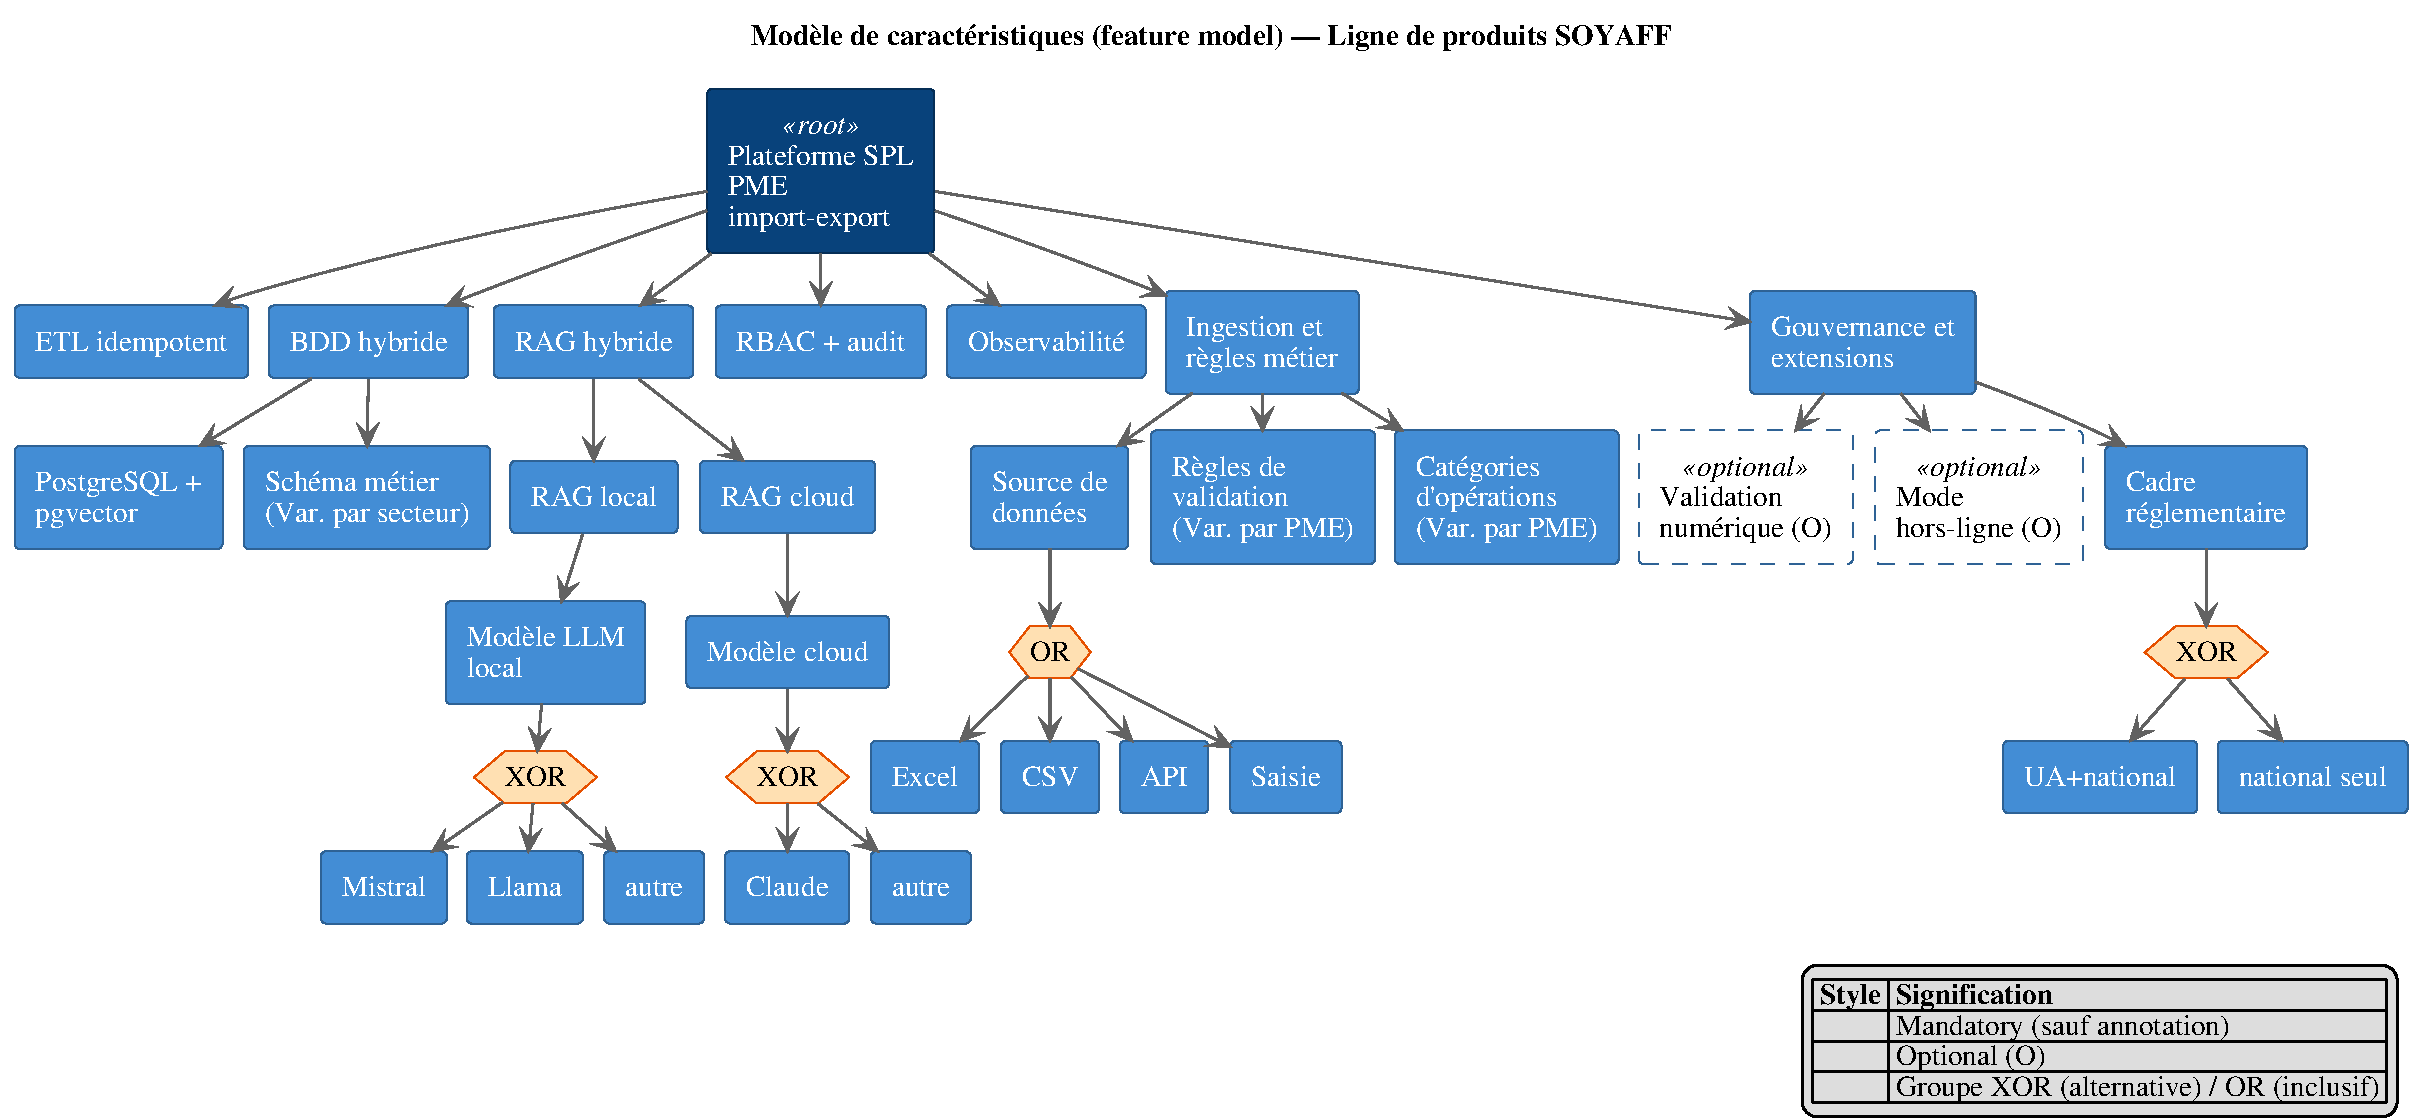
\includegraphics[width=\linewidth,height=0.85\textheight,keepaspectratio]{figures/fig_feature_model.pdf}
    \caption[Modèle de caractéristiques de la ligne de produits SOYAFF]{Modèle de caractéristiques (\textit{feature model}) de la ligne de produits SOYAFF. Sauf annotation contraire, une caractéristique est obligatoire.}
    \label{fig:feature_model_spl}
    \source{Schéma de l'auteur}
\end{figure}
\end{landscape}

Toutes les branches de premier niveau sont obligatoires. Trois d'entre elles (ETL idempotent, RBAC et audit, supervision) n'ont aucune variabilité. Les autres ne varient que dans leurs feuilles, jamais dans leur existence. C'est l'argument central pour H4 : la réutilisation est forte, et la variabilité est bornée à quelques points identifiés. Une contrainte n'apparaît pas dans l'arbre : le RAG local \emph{requiert} un moteur d'inférence local, donc le conteneur Ollama.

\subsection{Instanciation illustrative : SODRAF SARL (Bamako, Mali)}
\label{sec:spl_instanciation}

Pour rendre l'analyse concrète, nous dérivons sur le papier un second produit pour SODRAF SARL. Cette société de commerce d'import-export de produits alimentaires (riz, sucre, boissons), basée à Bamako, emploie de 51 à 200 personnes et est \textbf{partenaire commercial de SOYAFF} sur le corridor. Il s'agit d'une dérivation analytique, pas d'un déploiement.

\textbf{Ce qui est repris tel quel.} SODRAF gère elle aussi ses opérations sur des supports hétérogènes. Les six invariants sont repris sans modification : mêmes conteneurs, même topologie, même routage hybride.

\textbf{Ce qui est reconfiguré.}
\begin{itemize}
    \item \textbf{Le schéma métier.} Les camions, bons de livraison et chauffeurs laissent la place aux fournisseurs, produits, stocks et points de vente. C'est une modélisation de domaine à part entière, pas un paramétrage.
    \item \textbf{Le cadre juridique.} SODRAF relève du régime malien, hors Convention de Malabo : le socle juridique change de nature.
    \item \textbf{Les catégories et les règles métier.} Les catégories du transport (carburant, ration, frais de route) deviennent celles du commerce (achat, stockage, distribution, pertes) ; les contrôles de délai sont remplacés par des seuils de réapprovisionnement ou de péremption.
\end{itemize}

Aucun conteneur du plan applicatif, IA ou données (Tableau~\ref{tab:inventaire_conteneurs}) n'est remplacé ni supprimé. La charge réelle de reconfiguration du schéma n'a cependant pas été mesurée, et rien ne garantit qu'elle resterait contenue en pratique.

\subsection{Portée, limites et verdict sur H4}
\label{sec:spl_limites}

\textbf{Verdict.} L'architecture présente un noyau de six invariants et une variabilité bornée à sept points identifiés ; la dérivation vers SODRAF ne modifie aucun conteneur. \textbf{H4 est étayée analytiquement} : la réplicabilité est plausible sans refonte majeure. Elle n'est ni validée ni infirmée par l'expérience.

\textbf{Limites.}
\begin{itemize}
    \item \textbf{Un seul produit réel.} SOYAFF est le seul membre de la ligne construit et exploité ; SODRAF n'est dérivée que sur le papier.
    \item \textbf{Une variabilité en partie théorique.} Le modèle local est écrit en dur dans le code : le changer demande une modification du code, pas une simple configuration.
    \item \textbf{Le schéma métier reste le point le plus large.} Changer de secteur, même vers un secteur voisin, demande une nouvelle modélisation du domaine.
    \item \textbf{Le cadre juridique change de nature d'un pays à l'autre}, ce qui nuance l'idée d'une variabilité uniformément bornée.
\end{itemize}

La validation par un déploiement réel, chez SODRAF de préférence, est la suite logique de ce travail (section~\ref{chap:perspectives}).

\subsection{Synthèse et transition}
\label{sec:spl_synthese_transition}

H4 est étayée par l'analyse, pas encore démontrée par un second cas. Les quatre hypothèses ont maintenant été éprouvées : H2 par le benchmark, H1 et H3 par la mesure de l'impact, H4 par le raisonnement. Il reste à chiffrer le retour sur investissement (\S\ref{sec:roi}) et à répondre à la problématique (\S\ref{sec:reponse_problematique}).


\section{Retour sur investissement}
\label{sec:roi}

Cette section chiffre ce que la plateforme rapporte à SOYAFF, en FCFA. Nous ne valorisons pas des suppressions de postes : aucun emploi n'est supprimé. Le gain est du temps de travail libéré, valorisé au coût de la personne qui le récupère. Nous distinguons ce qui a été mesuré de ce qui est déclaré.

\subsection{Coûts}
\label{sec:roi_couts}

\textbf{Investissement initial.} Nous avons proposé à SOYAFF de facturer le développement de la plateforme 2~000~000~FCFA. Cette proposition n'est pas encore conclue ; nous la retenons comme valeur de l'investissement, celle qu'une entreprise paierait pour un projet équivalent.

\textbf{Coûts de fonctionnement.} Le Tableau~\ref{tab:roi_couts} détaille les dépenses mensuelles, converties au taux du 27~septembre~2026 (1~USD~=~598,02~FCFA).

\begin{table}[H]
\centering
\footnotesize
\caption{Coûts mensuels de fonctionnement de la plateforme}
\label{tab:roi_couts}
\begin{tabularx}{\linewidth}{|>{\raggedright\arraybackslash}X|r|r|}
\hline
\rowcolor[HTML]{EFEFEF}
\textbf{Poste} & \textbf{Montant facturé} & \textbf{Coût mensuel (FCFA)} \\ \hline
Serveur dédié OneProvider (sauvegarde de 100~Go incluse) & 30,23~USD par mois & 18~078 \\ \hline
API Anthropic (chemin cloud) & $\approx$~10~USD par mois & 5~980 \\ \hline
Nom de domaine & 10~USD par an & 498 \\ \hline
Logiciels (PostgreSQL, Airflow, n8n, Grafana, Docker\ldots) & 0 & 0 \\ \hline
\textbf{Total mensuel} & \textbf{41,06~USD} & \textbf{24~557} \\ \hline
\textbf{Total annuel} & & \textbf{294~680} \\ \hline
\end{tabularx}
\end{table}

\subsection{Gains}
\label{sec:roi_gains}

\textbf{Gain mesuré : la saisie à Dakar.} Le chronométrage du §\ref{sec:impact_temps} établit qu'une opération prend 11,16~minutes dans Excel et 1,71~minute sur la plateforme, soit 9,45~minutes gagnées. La base de production compte 4~756 transactions sur seize mois, soit environ 297 opérations par mois. L'agent de saisie récupère donc près de 47~heures par mois. Payé 400~000 à 500~000~FCFA par mois pour 173~heures de travail, son heure coûte 2~308 à 2~885~FCFA. Le temps libéré vaut ainsi \textbf{108~000 à 135~000~FCFA par mois}.

\textbf{Gain déclaré : la fin de la double saisie à Bamako.} Le chef logistique ne ressaisit plus les récapitulatifs envoyés de Dakar. Ce gain n'a pas été chronométré. Le chef logistique l'estime à deux heures par jour : la ressaisie lui prenait, selon ses mots, une bonne partie de la journée. Payé plus de 500~000~FCFA par mois, il récupère environ 43~heures mensuelles, soit au moins \textbf{125~000~FCFA par mois}. Nous présentons ce gain comme une estimation déclarée, non comme une mesure.

\subsection{Retour sur investissement}
\label{sec:roi_calcul}

Le Tableau~\ref{tab:roi_scenarios} présente deux scénarios. Le scénario~A ne retient que le gain mesuré à Dakar : c'est le plancher, que le jury peut vérifier sur les données du §\ref{sec:impact_temps}. Le scénario~B y ajoute le gain déclaré à Bamako.

\begin{table}[H]
\centering
\footnotesize
\caption{Retour sur investissement selon deux scénarios (297 opérations par mois)}
\label{tab:roi_scenarios}
\begin{tabularx}{\linewidth}{|>{\raggedright\arraybackslash}X|r|r|}
\hline
\rowcolor[HTML]{EFEFEF}
\textbf{Indicateur (FCFA)} & \textbf{A : mesuré} & \textbf{B : mesuré + déclaré} \\ \hline
Gain mensuel & 108~000 à 135~000 & 233~000 à 260~000 \\ \hline
Coût mensuel & 24~557 & 24~557 \\ \hline
\textbf{Gain net mensuel} & \textbf{83~000 à 110~000} & \textbf{208~000 à 235~000} \\ \hline
\textbf{Amortissement de 2~000~000~FCFA} & \textbf{18 à 24 mois} & \textbf{8,5 à 9,6 mois} \\ \hline
\end{tabularx}
\end{table}

Dans les deux scénarios, la plateforme rapporte plus qu'elle ne coûte dès le premier mois d'exploitation : le gain mensuel représente quatre à dix fois le coût de fonctionnement. Ce qui varie, c'est le délai pour rembourser l'investissement initial : moins de dix mois si l'on compte le gain de Bamako, un an et demi à deux ans sur le seul gain mesuré.

\textbf{Projection sur trois ans.} Le Tableau~\ref{tab:roi_projection} suit les deux scénarios année par année, pour un agent payé 450~000~FCFA (milieu de la fourchette).

\begin{table}[H]
\centering
\footnotesize
\caption{Projection financière sur trois ans (agent à 450~000~FCFA par mois)}
\label{tab:roi_projection}
\begin{tabular}{|l|r|r|r|r|}
\hline
\rowcolor[HTML]{EFEFEF}
\textbf{Année} & \textbf{Investissement} & \textbf{Coûts} & \textbf{Bilan cumulé A} & \textbf{Bilan cumulé B} \\ \hline
Année 1 & 2~000~000 & 294~680 & $-$837~381 & 662~619 \\ \hline
Année 2 & 0 & 294~680 & 325~237 & 3~325~237 \\ \hline
Année 3 & 0 & 294~680 & 1~487~856 & 5~987~856 \\ \hline
\end{tabular}
\end{table}

Sur trois ans, le bilan cumulé atteint environ 1,49~million de FCFA dans le scénario~A et 5,99~millions dans le scénario~B. Le volume d'opérations joue fortement : avec les 438 opérations de mars~2026 au lieu de la moyenne de 297, l'amortissement du scénario~B tombe à 7,2~mois.

\textbf{Ce que ce calcul ne compte pas.} Trois bénéfices ne sont pas valorisés, faute de mesure fiable : la réduction des erreurs de saisie (§\ref{sec:impact_erreurs}), la disponibilité de l'information en temps réel pour les décideurs, et le temps gagné par l'assistant conversationnel sur les analyses. Le retour sur investissement présenté ici est donc un minimum. À l'inverse, il suppose que le temps libéré est réemployé à des tâches utiles ; s'il ne l'est pas, le gain reste réel pour les personnes, mais pas pour la trésorerie.

\section{Réponse à la problématique}
\label{sec:reponse_problematique}

La problématique posée en introduction demandait comment concevoir, déployer et valider une architecture logicielle hybride et réplicable pour digitaliser une PME d'import-export ouest-africaine, sous des contraintes de budget, de connectivité et de souveraineté des données. Le Tableau~\ref{tab:reponse_questions} reprend les quatre questions de recherche qui la déclinent ; les paragraphes qui suivent y répondent une à une.

\begin{table}[H]
\centering
\footnotesize
\caption{Réponse aux questions de recherche}
\label{tab:reponse_questions}
\begin{tabularx}{\linewidth}{|l|>{\raggedright\arraybackslash}X|l|}
\hline
\rowcolor[HTML]{EFEFEF}
\textbf{Question} & \textbf{Réponse établie} & \textbf{Hypothèse} \\ \hline
Q1 : quelle architecture ? & Une plateforme mono-serveur (ETL, application web, IA hybride, DevOps), en production, pour 37,4~€ par mois & H1 confirmée \\ \hline
Q2 : le RAG local vaut-il le cloud ? & Non : 20~\% d'exactitude contre 88,9~\% & H2 réfutée \\ \hline
Q3 : quel impact métier, à quel coût ? & Environ 85~\% de temps de saisie en moins, investissement amorti en 8,5 à 24 mois & H3 confirmée (volet temps) \\ \hline
Q4 : l'architecture se réplique-t-elle ? & Un noyau invariant et des points de variation identifiés, sans second déploiement & H4 étayée analytiquement \\ \hline
\end{tabularx}
\end{table}

\textbf{D'une chaîne de fichiers Excel à une plateforme d'aide à la décision.} Le point de départ était une chaîne de fichiers. L'agent de Dakar saisissait les opérations dans un récapitulatif journalier, les recopiait dans un récapitulatif mensuel, puis envoyait le fichier par WhatsApp. À Bamako, le chef logistique attendait ce fichier, le ressaisissait dans ses propres tableaux, et les deux bureaux s'appelaient longuement pour lever les incohérences. Le point d'arrivée est une plateforme où chaque opération est saisie une seule fois, contrôlée au moment de la saisie et visible aussitôt dans les deux bureaux, avec un assistant qui répond en langage naturel sur l'ensemble des données. C'est la première réponse à la problématique : l'architecture a été conçue et déployée, et elle tourne en production.

\textbf{Q1 et H1 : une architecture frugale et complète.} Un seul serveur dédié porte le pipeline ETL, l'application web, les deux chemins d'IA, l'intégration continue et la supervision, pour 41,06~USD par mois, soit 37,4~€ (§\ref{sec:impact_cout}). Le seuil de 50~€ est respecté avec une marge d'un quart. La contrainte budgétaire n'a donc pas imposé de renoncer à l'une des briques. La contrainte de connectivité, elle, n'est que partiellement traitée : l'application exige une connexion, et le mode hors-ligne reste à construire (§\ref{sec:limites_solution}).

\textbf{Q3 et H3 : un impact mesuré sur le travail quotidien.} Le temps de saisie d'une opération passe de 11,16 à 1,71~minutes, soit une réduction de l'ordre de 85~\% (§\ref{sec:impact_temps}). Les utilisateurs le formulent plus simplement. L'agent de saisie ne saisit plus qu'une fois : fini la copie du journalier vers le mensuel et l'envoi par WhatsApp. Le chef logistique n'attend plus de fichier pour travailler : il voit chaque opération dès qu'elle est saisie. Le score d'utilisabilité de 88,1 (§\ref{sec:adoption_resultats}) et les entretiens confirment cette utilité perçue. En valorisant le temps libéré, l'investissement de 2~000~000~FCFA est amorti en 8,5 à 24 mois selon le scénario retenu (§\ref{sec:roi}).

\textbf{Q2 et H2 : la souveraineté tient, l'exactitude locale non.} Le benchmark a été la principale déception de ce travail. Le RAG local n'atteint que 20~\% d'exactitude, loin des 88,9~\% du cloud (§\ref{sec:bench_resultats_globaux}), et H2 est réfutée. Ce résultat ne remet pas en cause le principe de souveraineté : le routage hybride fonctionne de bout en bout, et les questions sensibles ne quittent pas le serveur (§\ref{sec:test_bout_en_bout}). Ce qu'il remet en cause, c'est la méthode de récupération du chemin local. Chercher par similarité sémantique dans des données relationnelles, pour répondre à des questions d'agrégat, était inadapté : le diagnostic le montre question par question (§\ref{sec:bench_diagnostic}). La réponse n'est pas d'abandonner le chemin local, mais de lui donner la méthode qui réussit côté cloud : générer une requête SQL à partir de la question (\textit{text-to-SQL}), avec un modèle exécuté sur le serveur. C'est la principale perspective de ce travail.

\textbf{Q4 et H4 : une réplicabilité étayée, pas encore démontrée.} L'analyse par lignes de produits logiciels distingue un noyau invariant, valable pour toute PME du même type (le pipeline ETL, l'IA hybride, le déploiement frugal sur un seul serveur), et des points de variation configurables (le schéma de la base, les rôles d'accès, une partie des règles métier) (§\ref{sec:spl_invariants}, §\ref{sec:spl_variation}). La dérivation vers SODRAF, entreprise partenaire de SOYAFF, est restée sur le papier : le temps a manqué pour la déployer. H4 est donc étayée par le raisonnement, pas encore par un second cas réel.

\textbf{En réponse à la problématique.} Une PME d'import-export ouest-africaine peut être digitalisée par une architecture hybride conçue pour ses contraintes : le système existe, il est utilisé, il fait gagner du temps et il coûte moins de 50~€ par mois. L'hybride tient comme principe de souveraineté. Il ne tient pas encore comme promesse d'exactitude sur le chemin local, et le benchmark indique précisément quoi changer pour y parvenir.

\section{Limites de la solution}
\label{sec:limites_solution}

Les résultats de ce chapitre valent dans des limites que nous rassemblons ici. Chacune est détaillée dans la section qui l'a établie ; le chapitre~\ref{chap:discussion_perspectives} en tire les conséquences sans les répéter.

\textbf{Limites techniques.}
\begin{itemize}
    \item \textbf{Le chemin local n'est pas fiable pour l'analyse.} Il atteint 20~\% d'exactitude, et ses réponses SQL directes peuvent être fausses tout en paraissant certaines : une somme à la place d'un comptage, une plaque qui fait ignorer le reste de la question (§\ref{sec:bench_diagnostic}). H2 est réfutée.
    \item \textbf{Le classifieur de sensibilité reste lexical.} Un nom de chauffeur cité seul, sans le mot « chauffeur » ni plaque, n'est pas détecté et part vers le cloud. Le rôle en lecture seule de l'agent, qui n'a pas accès à la table \texttt{chauffeurs}, borne ce risque sans le supprimer (§\ref{sec:ia_routage}). La précision du classifieur n'a pas été mesurée.
    \item \textbf{Un seul serveur.} Une panne arrête tous les services ; le déploiement n'a pas de retour arrière automatique (§\ref{sec:devops_dettes}).
    \item \textbf{Deux exigences restent à construire} : le mode hors-ligne (\texttt{ENF-DISP-01}), alors que la connectivité est une contrainte du terrain, et le circuit de validation numérique (\texttt{EF-VAL-02}) (§\ref{sec:webapp_fonctionnalites_cibles_non_deployees}).
\end{itemize}

\textbf{Limites de la mesure.}
\begin{itemize}
    \item \textbf{Le benchmark a été exécuté sur le serveur lui-même.} Ses latences n'incluent pas le trajet réseau jusqu'au poste de l'utilisateur. Les verdicts ont été attribués par un seul annotateur, sur un corpus rédigé par le concepteur du système (§\ref{sec:bench_limites}).
    \item \textbf{Le gain de temps repose sur cinq sessions rejouées} par un seul agent, avec un effet d'observation possible (§\ref{sec:impact_limites}). Le volet erreurs de H3 n'est que partiellement étayé : le seuil de 80~\% n'a pas pu être vérifié (§\ref{sec:impact_erreurs}).
    \item \textbf{L'adoption porte sur quatre utilisateurs.} C'est un recensement de tous les utilisateurs métier, pas un échantillon : le score SUS de 88,1 décrit ce cas, il ne se généralise pas (§\ref{sec:adoption_biais}).
    \item \textbf{Le gain de Bamako est déclaré, non mesuré}, et le retour sur investissement suppose que le temps libéré est réemployé (§\ref{sec:roi}).
    \item \textbf{La disponibilité est mesurable mais n'a pas été mesurée} sur une période significative (§\ref{sec:impact_cout}).
\end{itemize}

\textbf{Limites de contexte.}
\begin{itemize}
    \item \textbf{Un seul cas.} Toutes les mesures portent sur SOYAFF. H4 est étayée par un raisonnement sur les lignes de produits logiciels et une dérivation sur le papier vers une seconde PME, pas par un second déploiement (§\ref{sec:spl_limites}).
    \item \textbf{Des coûts en dollars.} Le serveur et l'API sont facturés en USD, alors que le franc CFA est arrimé à l'euro : le coût mensuel varie avec le taux de change.
    \item \textbf{Des données personnelles hors du serveur.} La copie de sauvegarde hors site n'est pas encore chiffrée (§\ref{sec:devops_dettes}), et les questions non sensibles, avec les résultats de l'agent, sont traitées par un service tiers.
\end{itemize}
